\let\negmedspace\undefined
\let\negthickspace\undefined
\documentclass[journal]{IEEEtran}
\usepackage[a5paper, margin=10mm, onecolumn]{geometry}
%\usepackage{lmodern} % Ensure lmodern is loaded for pdflatex
\usepackage{tfrupee} % Include tfrupee package

\setlength{\headheight}{1cm} % Set the height of the header box
\setlength{\headsep}{0mm}     % Set the distance between the header box and the top of the text

\usepackage{gvv-book}
\usepackage{gvv}
\usepackage{cite}
\usepackage{amsmath,amssymb,amsfonts,amsthm}
\usepackage{algorithmic}
\usepackage{graphicx}
\usepackage{textcomp}
\usepackage{xcolor}
\usepackage{txfonts}
\usepackage{listings}
\usepackage{enumitem}
\usepackage{mathtools}
\usepackage{gensymb}
\usepackage{comment}
\usepackage[breaklinks=true]{hyperref}
\usepackage{tkz-euclide} 
\usepackage{listings}
\usepackage{tikz}
\usetikzlibrary{patterns}
% \usepackage{gvv}                                        
\def\inputGnumericTable{}                                 
\usepackage[latin1]{inputenc}                                
\usepackage{color}                                            
\usepackage{array}                                            
\usepackage{longtable}                                       
\usepackage{calc}                                             
\usepackage{multirow}                                         
\usepackage{hhline}                                           
\usepackage{ifthen}                                           
\usepackage{lscape}
\usepackage{multicol}
\begin{document}

\bibliographystyle{IEEEtran}
\vspace{3cm}

\title{EE : Electrical Engineering}
\author{AI24BTECH11022 - Pabbuleti Venkata Charan Teja}
\maketitle

\renewcommand{\thefigure}{\theenumi}
\renewcommand{\thetable}{\theenumi}


\begin{enumerate}
\setcounter{enumi}{26}
\item An inductor having a $Q-$Factor of $60$ is connected in series with a capacitor having a $Q-$factor of $240$. The overall $Q-$factor of the circuit is \rule{1cm}{0.15mm} (round off to nearest integer) \hfill(2022)


\item The network shown below has a resonant frequency of $150kHz$ and a bandwidth of $600Hz$. The $Q-$factor of the network is \rule{1cm}{0.15mm} (round off to nearest integer) \hfill(2022)

\begin{tikzpicture}[scale=0.75]
\def\radius{2}
\def\smallradius{1.414}
\foreach \angle [count=\i] in {0,45,...,315} {
\coordinate (A\i) at (\angle+22.5:\radius);
}
\foreach \i [remember=\i as \lasti (initially 8)] in {7} {
\fill[gray!30] (0,0) -- (A\i) -- (A\lasti) -- cycle;
}
\foreach \i [remember=\i as \lasti (initially 5)] in {4,3} {
\fill[gray!30] (0,0) -- (A\i) -- (A\lasti) -- cycle;
}

\foreach \i [remember=\i as \lasti (initially 8)] in {1,...,8} {
\draw (A\lasti) -- (A\i);
}
\begin{scope}[shift={(2.2,-2.2)}]
\foreach \angle [count=\i] in {0,60,...,300} {
\coordinate (B\i) at (\angle+45:\smallradius);
}
\foreach \i [remember=\i as \lasti (initially 6)] in {1,2} {
\fill[gray!30] (0,0) -- (B\i) -- (B\lasti) -- cycle;
}
\foreach \i [remember=\i as \lasti (initially 6)] in {1,...,6} {
\draw (B\lasti) -- (B\i);
}
\end{scope}
\draw[dashed,thick] (4,-4) -- (4,2.5);
\end{tikzpicture}


\item The maximum clock frequency in $MHz$ of a $4-$stage ripple counter, utilizing flip-flops, with each flip-flop having a propagation delay of $20ns$, is \rule{1cm}{0.15mm}. (round off to one decimal place) \hfill(2022)


\item If only $5\%$ of the supplied power to a cable reaches the output terminal, the power loss in the cable, in $decibels$, is \rule{1cm}{0.15mm}. (round off to nearest integer) \hfill(2022)


\item In the circuit shown below, the switch $S$ is closed at $t=0$. The magnitude of the steady state voltage, in $volts$, across the $6\ohm$ resistor is \rule{1cm}{0.15mm}. (round off to two decimal places) \hfill(2022)

\begin{circuitikz}
\draw (5,0) to [R=$2\ohm$] (3,0) to [closing switch, l=S] (2,0) to [battery1,l=$10V$] (0,0) -- (0,1) to [C=$1\micro F$] (2.5,1) to [R=$10\ohm$] (5,1);
\draw (4,3) -- (5,3) -- (5,0);
\draw (0,0) -- (0,3) -- (1,3) -- (1,3.5) to [R=$6\ohm$] (4,3.5) -- (4,2.5) to [R=$3\ohm$] (1,2.5) -- (1,3);
\end{circuitikz}


\item A single-phase full-bridge diode rectifier feeds a resistive load of $50\ohm$ from a $200V$, $50Hz$ single phase $AC$ supply. If the diodes are ideal, then the active power, in $watts$, drawn by the load is \rule{1cm}{0.15mm}. (round off to nearest integer) \hfill(2022)


\item The voltage at the input of an AC-DC rectifier is given by $v\brak{t}=230\sqrt{2}sin{\omega t}$ where $\omega=2\pi\times 50rad/s$. The input current drawn by the rectifier is given by $$i\brak{t}=10\sin{\brak{\omega t-\frac{\pi}{3}}}+4\sin{\brak{3\omega t-\frac{\pi}{6}}}+3\sin{\brak{5\omega t-\frac{\pi}{3}}}$$ The input power factor, (rounded off to two decimal places), is, \rule{1cm}{0.15mm} lag. \hfill(2022)


\item Two balanced three-phase loads, as shown in the figure, are connected to a $100\sqrt{3}V$, three-phase, $50Hz$ main supply Given $Z_{1}=(18+j24)\ohm$ and $Z_{2}=\brak{6+j8}\ohm$. The ammeter reading, in amperes, is \rule{1cm}{0.15mm}. (round off to nearest integer) \hfill(2022)

\begin{tikzpicture}
\foreach \x in {-2,-1,0,1,2} {
\draw[->] (0,\x/2) -- (1,\x/2);
}
\draw[<->] (-0.2,-1) -- (-0.2,0) node[midway,left] {$H_{U}$};
\draw[<->] (-0.2,1) -- (-0.2,0) node[midway,left] {$H_{U}$};
\node at (0.5,1.25) {$u=U_{\infty}$};
\draw[dashed] (1,-0.5) -- (1,1);
\draw (1,-0.75) circle (0.2cm);
\node at (1,-0.75) {$1$};
\draw[->] (1.1,0) -- (1.75,0) node[right] {$x$};
\draw[->] (1.1,0) -- (1.1,0.75) node[right] {$y$};
\draw[dashed] (1,1) parabola (1.25,1.25);
\draw[dashed] (1,-1) parabola (1.25,-1.25);
\draw[dashed] plot[smooth,domain=1:2] ({\x^2+0.25},\x+0.25);
\draw[dashed] plot[smooth,domain=1:2] ({\x^2+0.25},-\x-0.25);
\draw (4.45,2.25) circle (0.2cm);
\node at (4.45,2.25) {$3$};
\draw (4.45,-2.25) circle (0.2cm);
\node at (4.45,-2.25) {$2$};
\draw[dashed] plot[smooth,domain=2.1:2.5] ({\x^2+0.25},\x+0.25);
\draw[dashed] plot[smooth,domain=2.1:2.5] ({\x^2+0.25},-\x-0.25);
\draw[dashed] (6.5,2.75) -- (9,2.75);
\draw[dashed] (6.5,-2.75) -- (9,-2.75);
\draw[<->] (8.75,0) -- (8.75,2.75) node[midway,left] {$H_{D}=0.03c$};
\draw[<->] (8.75,0) -- (8.75,-2.75) node[midway,left] {$H_{D}=0.03c$};
\draw[dashed] (9.25,-2.15) -- (9.25,2.75);
\draw[dashed] (9.25,-2.75) -- (9.25,-2.55);
\draw (9.25,-2.35) circle (0.2cm);
\node at (9.25,-2.35) {$4$};
\draw (10,2.75) -- (9.25,0) node[midway,right] {$u=\brak{y/H_{D}}U_{\infty}$} -- (10,-2.75) node[midway,right] {$u=\brak{-y/H_{D}}U_{\infty}$};
\draw[->] (9.25,-2.75) -- (10,-2.75);
\draw[->] (9.25,-2) -- (9.8,-2);
\draw[->] (9.25,-1.25) -- (9.6,-1.25);
\draw[->] (9.25,2.75) -- (10,2.75);
\draw[->] (9.25,2) -- (9.8,2);
\draw[->] (9.25,1.25) -- (9.6,1.25);
\node at (6.5,3) {streamline};
\node at (6.5,-3) {streamline};
\draw[<->] (3,-0.5) -- (5,-0.5) node[midway,above] {$c$};
\draw (4,0) ellipse (1cm and 0.15cm);
\end{tikzpicture}


\item The frequencies of the stator and rotor currents flowing in a three-phase $8-$pole induction motor are $40Hz$ and $1Hz$, respectively. The motor speed, in rpm, is \rule{1cm}{0.15mm}. (round off to nearest integer) \hfill(2022)


\item The output impedance of a non-ideal operational amplifier is denoted by $Z_{out}$. The variation in the magnitude of $Z_{out}$ with increasing frequency, $f$, in the circuit shown below, is best represented by \hfill(2022)

\begin{circuitikz}
\draw (2,2) node[op amp] (opamp) {};
\draw (0,0) to[sV, l=$V_{\text{in}}$] (0,1.5) -- (opamp.+);
\draw (opamp.-) |- (1,3.5) -| (opamp.out);
\draw[-o] (opamp.out) -- ++(1,0) node[right] {$V_{\text{out}}$};
\draw (0,0) -- (0,-0.1) node[ground] {};
\end{circuitikz}
\begin{multicols}{2}
\begin{enumerate}
\item \begin{tikzpicture}
\draw[->] (0,0) -- (1,0) node[right] {$\log\brak{f}$};
\draw[->] (0,0) -- (0,1) node[above] {$\log\brak{\abs{Z_{out}}}$};
\draw (0,0.75) -- (0.75,0.75);
\end{tikzpicture}
\item \begin{tikzpicture}
\draw[->] (0,-1) -- (0,1) node[above] {North};
\draw[->] (-1,0) -- (1,0) node[right] {East};
\end{tikzpicture}
\item \begin{tikzpicture}
\draw (-1,0) node[left,below] {$P$} -- (1,0) node[right,below] {$Q$} -- (1.62,1.18) node[right] {$R$} -- (0,1.9) node[above] {$S$} -- (-1.62,1.18) node[left] {$T$} -- (-1,0);
\end{tikzpicture}
\item \begin{tikzpicture}
\draw (-0.5,-0.866) node[below,left] {$P$} -- (0.5,-0.866) node[below,right] {$Q$} -- (1,0) node[right] {$R$} -- (0.5,0.866) node[above,right] {$S$} -- (-0.5,0.866) node[above,left] {$T$} -- (-1,0) node[left] {$U$} -- (-0.5,-0.866);
\end{tikzpicture}
\end{enumerate}
\end{multicols}


\item An $LTI$ system is shown in the figure where $G\brak{s}=\frac{100}{s^{2}+0.1s+10}$. The steady state output of the system, to the input $r\brak{t}$, is given as $y\brak{t}=a+b\sin{\brak{10t+\theta}}$. The values of '$a$' and '$b$' will be \hfill(2022)

\begin{tikzpicture}
\draw[->] (0,1) -- (1,1);
\draw (1,1) -- (2,1);
\draw (2,0) rectangle (5,2);
\draw[->] (5,1) -- (6,1);
\draw (6,1) -- (7,1);
\node[above] at (0,1) {$r\brak{t}=1+0.1\sin{\brak{10t}}$};
\node[above] at (6,1) {$y\brak{t}$};
\node at (3.5,1) {$G\brak{s}$};
\end{tikzpicture}
\begin{multicols}{2}
\begin{enumerate}
\item $a=1$, $b=10$
\item $a=10$, $b=1$
\item $a=1$, $b=100$
\item $a=100$, $b=1$
\end{enumerate}
\end{multicols}


\item The open loop transfer function of a unity gain negative feedback system is given as $G\brak{s}=\frac{1}{s\brak{s+1}}$. The Nyquist contour in the $s-$plane encloses the entire right half plane and a small neighbourhood around the origin in the left half plane, as shown in the figure below. The number of encirclements of the point $\brak{-1+j0}$ by the Nyquist plot of $G\brak{s}$, corresponding to the Nyquist contour, is denoted as $N$. Then $N$ equals to \hfill(2022)

\begin{tikzpicture}
\draw (0,0) node[below] {$Q$} -- (0.43,1.49) node[above] {$T$} -- (-0.87,0.34) node[below,left] {$P$} -- (1.05,1.02) node[right] {$R$} -- (-1.05,1.02) node[left] {$W$} -- (0.87,0.34) node[below,right] {$S$} -- (-0.43,1.49) node[above] {$U$} -- (0,0);
\end{tikzpicture}
\begin{multicols}{2}
\begin{enumerate}
\item $0$
\item $1$
\item $2$
\item $3$
\end{enumerate}
\end{multicols}


\item The damping ratio and undamped natural frequency of a closed loop system as shown in the figure, are denoted as $\zeta$ and $w_{n}$, respectively. The values of $\zeta$ and $w_{n}$ are \hfill(2022)

\begin{tikzpicture}
\draw[->] (0,3) -- (0.5,3) node[midway,above] {$R\brak{s}$};
\draw (0.5,3) -- (0.9,3);
\draw[->] (1.1,3) -- (1.9,3);
\draw (1.9,3) -- (2.9,3);
\draw[->] (3.1,3) -- (4,3);
\draw (3.5,3) -- (4.5,3);
\draw (4.5,2.5) rectangle (5.5,3.5);
\draw[->] (5.5,3) -- (7.25,3);
\draw (7,3) -- (7.5,3);
\draw (7.5,2.5) rectangle (8.5,3.5);
\draw[->] (8.5,3) -- (9.5,3) node[right,above] {$Y\brak{s}$};
\draw (1,3) circle (0.1cm);
\draw (3,3) circle (0.1cm);
\draw[->] (6.5,3) -- (6.5,2);
\draw (6.5,2) -- (6.5,1.5);
\draw (6.5,1.5) -- (3,1.5);
\draw[->] (3,1.5) -- (3,2.9);
\draw[->] (9,3) -- (9,1.5);
\draw (9,1.5) -- (9,1);
\draw (9,1) -- (1,1);
\draw[->] (1,1) -- (1,2.9);
\node at (5,3) {$10/s$};
\node at (8,3) {$10/s$};
\node at (0.8,3.2) {$+$};
\node at (0.75,2.8) {$-$};
\node at (2.8,3.2) {$+$};
\node at (2.75,2.8) {$-$};
\end{tikzpicture}
\begin{multicols}{2}
\begin{enumerate}
\item $\zeta=0.5$ and $w_{n}=10rad/s$
\item $\zeta=0.1$ and $w_{n}=10rad/s$
\item $\zeta=0.707$ and $w_{n}=10rad/s$
\item $\zeta=0.707$ and $w_{n}=100rad/s$
\end{enumerate}
\end{multicols}
\end{enumerate}
\end{document}